
\chapter{Testing and results}
\section{Testing the Code}
After testing the code, these are the results that we came to. 

As we can see in the beginning, the process actively requests input from the user in order to proceed with the implementation. It started by asking the user for login credentials, then the Project ID that the user wants to process, and lastly, before proceeding with the creation and command sending to XNAT, it asked the user about the command name and the description.
After receiving all the information, the script commenced building the image, tagging, pushing, writing the JSON command, enabling the command, and lastly launching the container with all files.

\section{Results on XNAT}
The result that we came to after testing the code is that all the steps are working correctly, except that the container could not receive any files. With the \ac{STDout} view we found out that the container received zero files. 
 
\begin{figure}
    \centering
    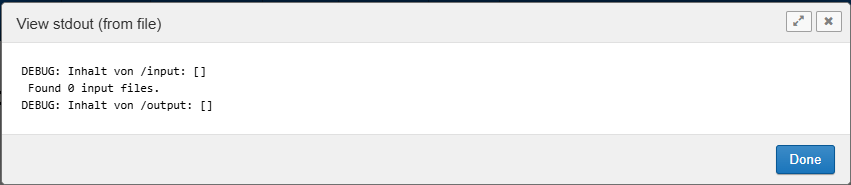
\includegraphics[width=0.9\textwidth]{en/content/STDOUT view.png}
    \caption{The STDout view of the container on XNAT}
    \label{fig:enter-label}
\end{figure}

But interestingly, after searching in the container information, we noticed that the container in fact received the files and that the files are listed in the input part of the container input. 

\begin{figure}[p]
    \centering
    \rotatebox{90}{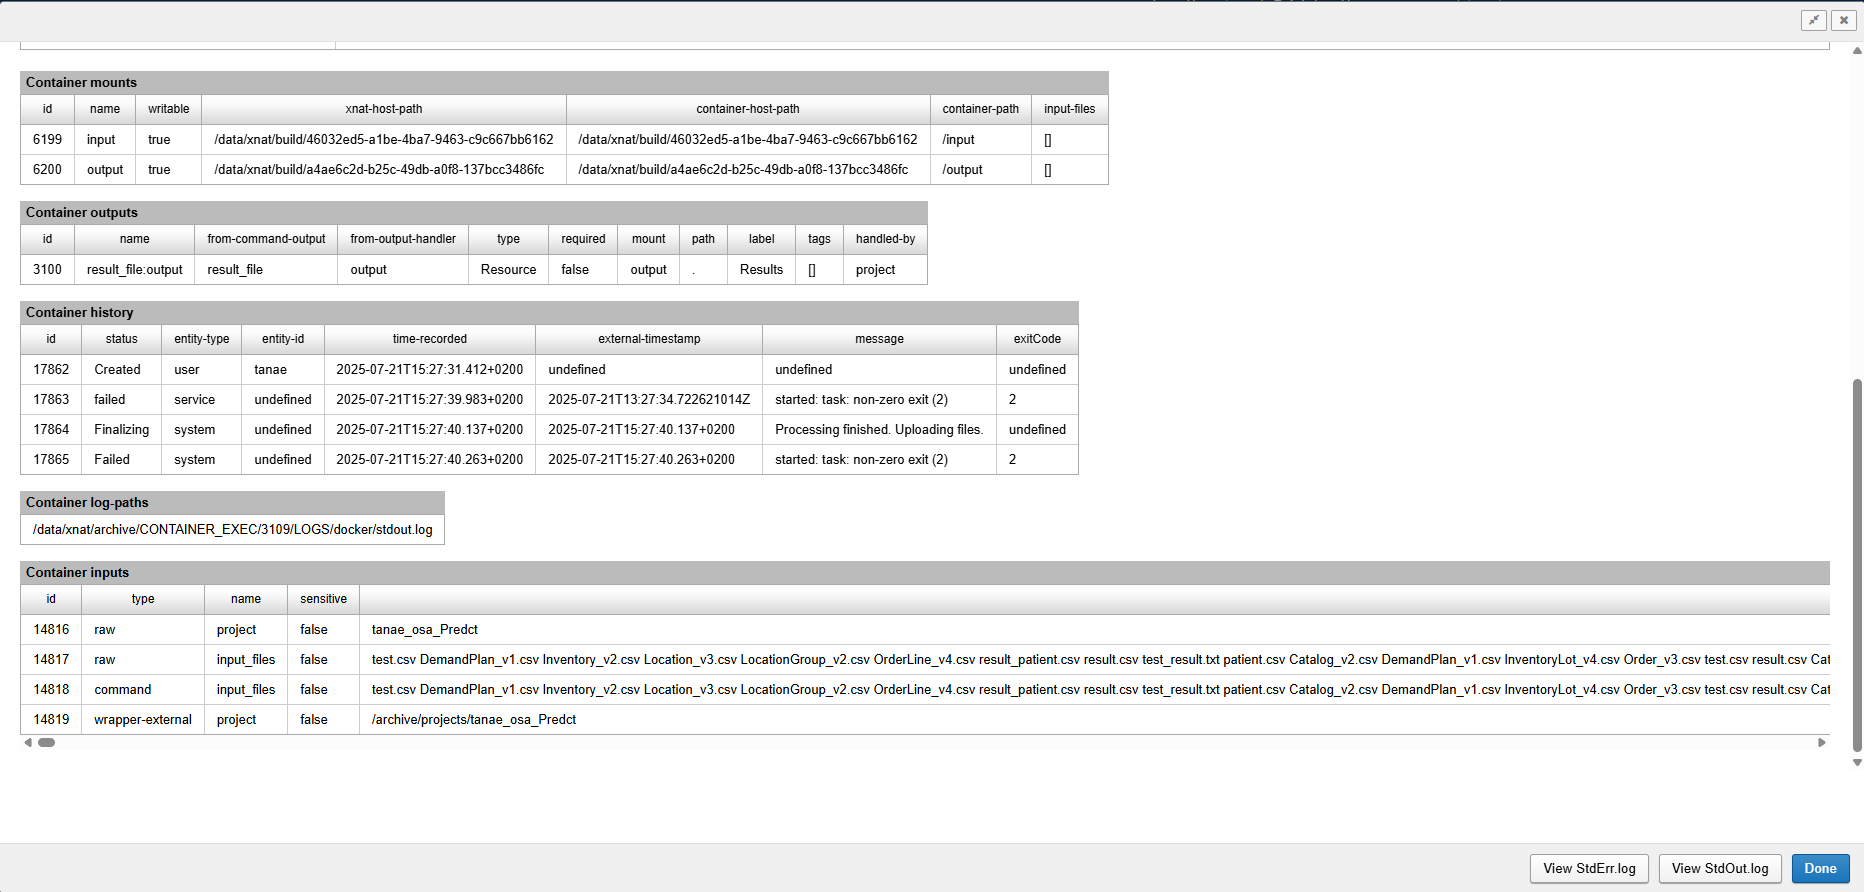
\includegraphics[width=0.95\textheight]{en/content/Container informatin 1.png}}
    \caption{Container Information 1}
    \label{fig:container-info-1}
\end{figure}

\begin{figure}
    \centering
    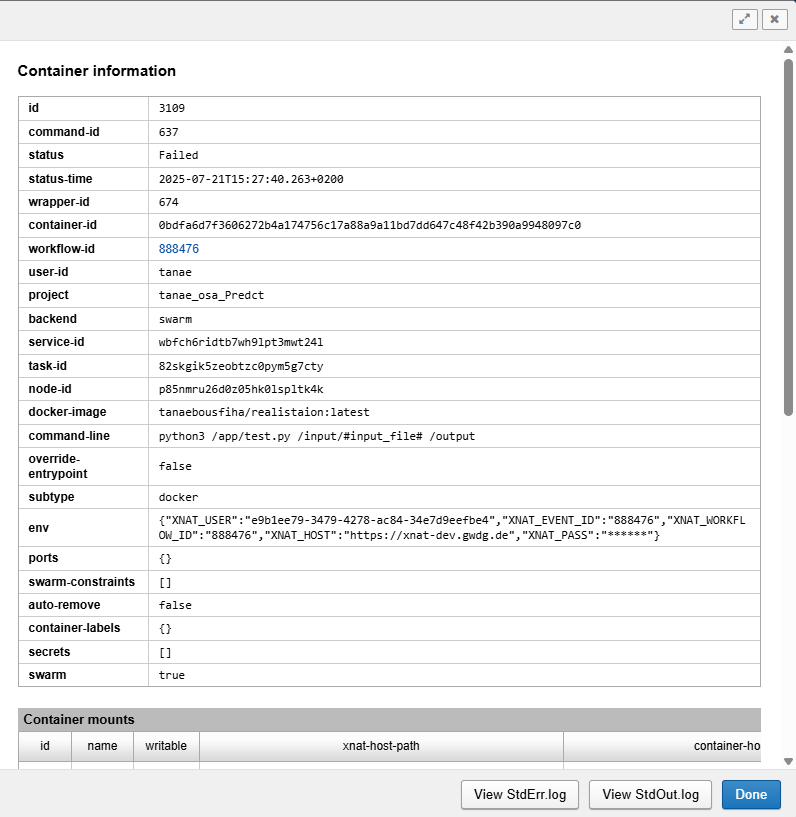
\includegraphics[width=0.9\linewidth]{en/content/Container information 2.png}
    \caption{Container Information 2}
    \label{fig:enter-label}
\end{figure}

Details of the test procedure are described in Appendix A \cite{bousfiha2025appendix}.

The results demonstrate two things. First, the automation script with the REST API worked correctly. Second, there is an issue with the container accessing the input files, despite them being listed as received.
